\documentclass[letterpaper,11pt]{article}

\usepackage{latexsym}
\usepackage[empty]{fullpage}
\usepackage{titlesec}
\usepackage{marvosym}
\usepackage[usenames,dvipsnames]{color}
\usepackage{verbatim}
\usepackage{enumitem}
\usepackage[hidelinks]{hyperref}
\usepackage{fancyhdr}
\usepackage[english]{babel}
\usepackage{tabularx}
\usepackage{fontawesome5}
\usepackage{multicol}
\setlength{\multicolsep}{-3.0pt}
\setlength{\columnsep}{-1pt}
\input{glyphtounicode}

%new packages

\usepackage{fontenc}
\usepackage{amsmath}
\usepackage{amssymb}
\usepackage{graphicx}



%----------FONT OPTIONS----------

\pagestyle{fancy}
\fancyhf{} % clear all header and footer fields
\fancyfoot{}
\renewcommand{\headrulewidth}{0pt}
\renewcommand{\footrulewidth}{0pt}

% Adjust margins
\addtolength{\oddsidemargin}{-0.6in}
\addtolength{\evensidemargin}{-0.5in}
\addtolength{\textwidth}{1.19in}
\addtolength{\topmargin}{-.7in}
\addtolength{\textheight}{1.4in}

\urlstyle{same}

\raggedbottom
\raggedright
\setlength{\tabcolsep}{0in}

% Sections formatting
\titleformat{\section}{
  \vspace{-4pt}\scshape\raggedright\large\bfseries
}{}{0em}{}[\color{black}\titlerule \vspace{-5pt}]



% Ensure that generate pdf is machine readable/ATS parsable
\pdfgentounicode=1

%-------------------------
% Custom commands
\newcommand{\resumeItem}[1]{
  \item\small{
    {#1 \vspace{-2pt}}
  }
}

\newcommand{\classesList}[4]{
    \item\small{
        {#1 #2 #3 #4 \vspace{-2pt}}
  }
}

\newcommand{\resumeSubheading}[4]{
  \vspace{-2pt}\item
    \begin{tabular*}{1.0\textwidth}[t]{l@{\extracolsep{\fill}}r}
      \textbf{#1} & \textbf{\small #2} \\
      \textit{\small#3} & \textit{\small #4} \\
    \end{tabular*}\vspace{-7pt}
}

\newcommand{\resumeSubSubheading}[2]{
    \item
    \begin{tabular*}{0.97\textwidth}{l@{\extracolsep{\fill}}r}
      \textit{\small#1} & \textit{\small #2} \\
    \end{tabular*}\vspace{-7pt}
}

\newcommand{\resumeProjectHeading}[2]{
    \item
    \begin{tabular*}{1.001\textwidth}{l@{\extracolsep{\fill}}r}
      \small#1 & \textbf{\small #2}\\
    \end{tabular*}\vspace{-7pt}
}


\newcommand{\resumeSubItem}[1]{\resumeItem{#1}\vspace{-4pt}}

\renewcommand\labelitemi{$\vcenter{\hbox{\tiny$\bullet$}}$}
\renewcommand\labelitemii{$\vcenter{\hbox{\tiny$\bullet$}}$}

\newcommand{\resumeSubHeadingListStart}{\begin{itemize}[leftmargin=0.0in, label={}]}
\newcommand{\resumeSubHeadingListEnd}{\end{itemize}}
\newcommand{\resumeItemListStart}{\begin{itemize}}
\newcommand{\resumeItemListEnd}{\end{itemize}\vspace{-5pt}}


\begin{document}
\fontfamily{cmr}\selectfont
\begin{center}
\parbox{3.0cm}{%
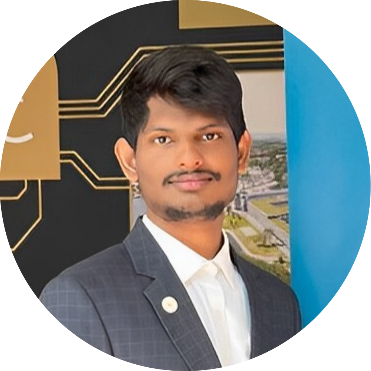
\includegraphics[width=2.7cm,clip]{images/resume_pic_m.png}}
}
\parbox{\dimexpr\linewidth-3.8cm\relax}{
\vspace{-20pt}
\begin{tabularx}{\linewidth}{L r} \\
    {\Huge \scshape  Venkata Sai Yakkshit Reddy Asodi}~
    \href{https://www.cedzlabs.com/yakkshit}{\vspace{1pt}}\\
      Zurich, Switzerland \\ \vspace{1pt}
     \small \raisebox{-0.1\height}\faPhone\ +41 0793550685 ~ \href{mailto:saiyakkshit2001@gmail.com}{\raisebox{-0.2\height}\faEnvelope\  {saiyakkshit2001@gmail.com}} ~ 
    \href{https://linkedin.com/in/yakkshit/}{\raisebox{-0.2\height}\faLinkedin\ {yakkshit}}  ~
    \href{https://yakkshit.com/}{\raisebox{-0.2\height}\faGlobe\ {yakkshit.com}}  ~
    \href{https://github.com/yakkshit}{\raisebox{-0.2\height}\faGithub{ yakkshit}}
    \vspace{-8pt}
\end{tabularx}
}
\end{center}

\vspace{-23pt}
\section{Summary \faLink}
Full Stack Developer with strong expertise in data engineering and visualization, specializing in building scalable web applications with Python and JavaScript. Proven track record in developing and maintaining data pipelines, creating interactive visualizations, and implementing machine learning solutions. Experienced in agile methodologies and cross-functional team collaboration, with a focus on delivering high-quality, maintainable code.

\section{\href{https://www.linkedin.com/in/yakkshit/details/skills/}{Technical Skills} \faLink}
\begin{itemize}[leftmargin=0.15in, label={}]
\small{\item{
\textbf{Languages - }{Python, JavaScript, SQL, HTML5, CSS3} \\
\textbf{Data Engineering - }{Databricks, pandas, numpy, scikit-learn} \\
\textbf{Visualization - }{Plotly, D3.js, Matplotlib} \\
\textbf{Tools \& Platforms - }{Git, Jira, Docker, AWS, Azure} \\
\textbf{Testing - }{pytest, Jest, Unit Testing}
}}
\end{itemize}
\vspace{-10pt}

\section{Experience \faLinkedin}
\resumeSubHeadingListStart

\resumeSubheading
{\large Circleup AG \faBuilding}{December 2023 -- Present}
{Lead Full Stack Engineer}{\faMapMarker \hspace{0.1cm} Zurich, Switzerland}\\
\vspace{10pt}
\textbf{Responsibilities:}
\resumeItemListStart
\vspace{-10pt}
\resumeItem{Developed and maintained data pipelines processing large-scale pharmaceutical data using Python and SQL, resulting in 40\% improved data processing efficiency.}
\resumeItem{Implemented interactive data visualizations using Plotly and D3.js for real-time monitoring of clinical trial metrics.}
\resumeItem{Created RESTful APIs for seamless integration of machine learning models with existing systems.}
\resumeItem{Led agile development teams using Jira for project management, consistently meeting sprint goals.}
\resumeItemListEnd
\vspace{-3pt}
\textbf{Environment:}\emph{Python, SQL, Plotly, REST APIs, Jira, Agile}

\resumeSubheading
{Cedzlabs \faBuilding}{March 2023 -- November 2023}
{Full Stack Developer}{\faMapMarker \hspace{0.1cm} India}\\
\vspace{10pt}
\textbf{Responsibilities:}
\vspace{-10pt}
\resumeItemListStart
\resumeItem{Built data processing pipelines using pandas and numpy, handling complex datasets for healthcare applications.}
\resumeItem{Developed automated testing frameworks ensuring 95\% code coverage for critical data operations.}
\resumeItemListEnd
\vspace{-3pt}
\textbf{Environment:}\emph{Python, pandas, numpy, pytest, SQL}

\section{Projects \faGithub}
\vspace{-5pt}
\resumeSubHeadingListStart

\resumeProjectHeading
{\textbf{\href{https://github.com/yakkshit}{Clinical Data Pipeline}} $|$ \emph{Python, Databricks, ML}}{2023}\\
\vspace{6pt}
\textbf{Description:}
\vspace{-5pt}
\resumeItemListStart
\resumeItem{Designed and implemented an end-to-end data pipeline using Databricks for processing clinical trial data. Integrated machine learning models for predictive analytics and created interactive dashboards using Plotly for real-time monitoring.}
\resumeItemListEnd
\vspace{4pt}
\textbf{Tools:}\emph{Python, Databricks, Plotly, scikit-learn, SQL}
\vspace{-10pt}

\resumeProjectHeading
{\textbf{\href{https://github.com/yakkshit}{Healthcare Analytics Platform}} $|$ \emph{Python, AWS}}{2023}\\
\vspace{6pt}
\textbf{Description:}
\vspace{-5pt}
\resumeItemListStart
\resumeItem{Developed a scalable analytics platform for healthcare data analysis, featuring automated ETL processes and interactive visualizations. Implemented unit testing framework achieving 90\% code coverage.}
\resumeItemListEnd
\vspace{4pt}
\textbf{Tools:}\emph{Python, AWS, SQL, Plotly, pytest}

\section{Achievements / Certifications}
\resumeItemListStart
\resumeItem{AWS Certified Developer Associate with focus on data engineering pipelines}
\resumeItem{Completed Advanced Data Engineering with Databricks certification}
\resumeItem{Led successful migration of legacy data systems to modern cloud infrastructure}
\resumeItemListEnd

\resumeSubHeadingListEnd
\textbf{Languages:}\emph{English - Fluent $|$ German - Elementary $|$ Hindi - Fluent}

\vspace{10pt}
\end{document}